\documentclass[10pt,executivepaper]{article}
\usepackage[utf8]{inputenc}
\usepackage[spanish]{babel}
\usepackage{amsmath}
\usepackage{amsfonts}
\usepackage{amssymb}
\usepackage{graphics}
\usepackage{graphicx}
\usepackage[left=2cm,right=2cm,top=2cm,bottom=2cm]{geometry}
\usepackage{imakeidx}
\makeindex[columns=3, title=Alphabetical Index, intoc]
\usepackage{listings}
\usepackage{xcolor}
\usepackage{multicol}
\usepackage{changepage}
\usepackage{float}
\usepackage{cite}
\usepackage{url}
\usepackage{pdflscape}
\usepackage{listingsutf8}

\definecolor{codegreen}{rgb}{0,0.6,0}
\definecolor{codegray}{rgb}{0.5,0.5,0.5}
\definecolor{codepurple}{rgb}{0.58,0,0.82}
\definecolor{backcolour}{rgb}{0.95,0.95,0.92}

\lstdefinestyle{mystyle}{
    backgroundcolor=\color{backcolour},
    commentstyle=\color{codegreen},
    keywordstyle=\color{magenta},
    numberstyle=\tiny\color{codegray},
    stringstyle=\color{codepurple},
    basicstyle=\ttfamily\footnotesize,
    breakatwhitespace=false,
    breaklines=true,
    captionpos=b,
    keepspaces=true,
    numbers=left,
    numbersep=5pt,
    showspaces=false,
    showstringspaces=false,
    showtabs=false,
    tabsize=3,
    inputencoding=utf8,
    extendedchars=true,
    literate={á}{{\'a}}1 {ñ}{{\~n}}1 {é}{{\'e}}1,
}

\def\fillandplacepagenumber{%
 \par\pagestyle{empty}%
 \vbox to 0pt{\vss}\vfill
 \vbox to 0pt{\baselineskip0pt
   \hbox to\linewidth{\hss}%
   \baselineskip\footskip
   \hbox to\linewidth{%
     \hfil\thepage\hfil}\vss}}


\lstset{style=mystyle}

\title{Actividad: Instalación de NFS en la nube}

\author{Instituto Politécnico Nacional\\Escuela Superior de Computo\\Desarrollo de Sistemas Distribuidos\\Adrian González Pardo\\4CV1\\21/01}
\date{\today}
\newcommand\tab[1][1cm]{\hspace*{#1}}

\begin{document}
% Portada
%encabezado
\begin{minipage}{0.4\textwidth}
	\begin{flushleft}
		
\includegraphics[scale = 0.05]{logoescom.png}
	\end{flushleft}
\end{minipage}
\begin{minipage}{0.51\textwidth}
	\begin{flushright}
		
\includegraphics[scale = 0.055]{logoipn.png}
	\end{flushright}
\end{minipage}
\begin{center}
	\par\vspace{0.5cm}{
	\huge\textbf{Instituto Politécnico Nacional \\*[0.20cm] Escuela Superior de Cómputo}}
\par\vspace{1cm}{
	\large\textbf{Desarrollo de Sistemas Distribuidos\\Actividad: Instalación de NFS en la nube\\Curso impartido por el profesor: Pineda Guerrero Carlos\\Grupo: 4CV1\\21/01\\Alumno: Adrian González Pardo\\}
}
\par\vspace{1cm}{
	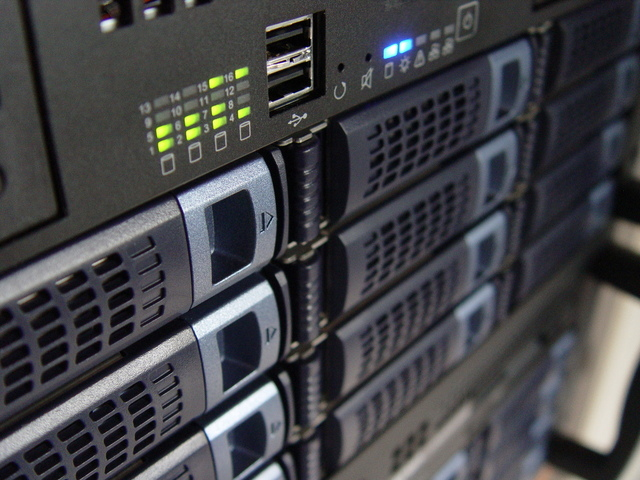
\includegraphics[scale=0.5]{servers.jpg}
}
\par\vspace{2cm}{
	Ultima fecha modificado: \today
}
\end{center}

% Indice
\clearpage
\section{Desarrollo}
Para esta práctica si bien no necesitamos de ningún lenguaje para programar estas tareas, nos apoyamos de un script en bash para la realización de la instalación configuración y muestra de datos solicitados en la práctica
\section{Códigos y scripts para funcionamiento}
\subsection{Script ejemplo clase:}
\lstinputlisting[language=Bash]{../script_first.sh}
\subsection{Script parte 1:}
\lstinputlisting[language=Bash]{../script_practica.sh}
\subsection{Script parte 2:}
\lstinputlisting[language=Bash]{../script_practica2.sh}
\section{Capturas}
\subsection{VM}
\begin{center}
  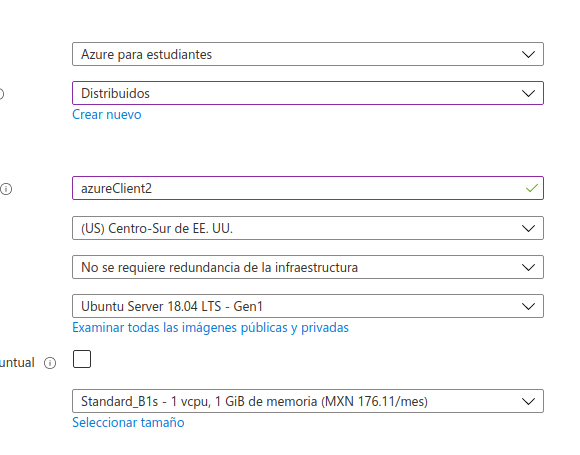
\includegraphics[scale=0.5]{imgs/creacion_0.png}\\
  \textit{Figura 1: Casillas de selección para la creación de la VM}\\
  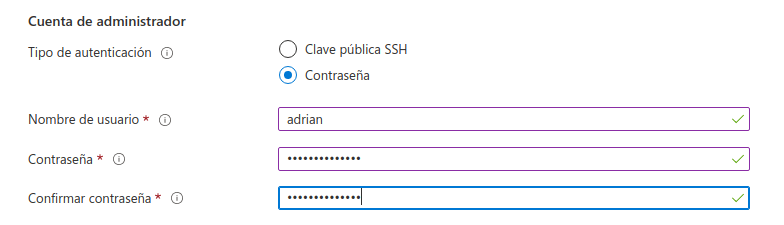
\includegraphics[scale=0.5]{imgs/creacion_1.png}\\
  \textit{Figura 2: Casillas de selección para la creación de la VM}\\
  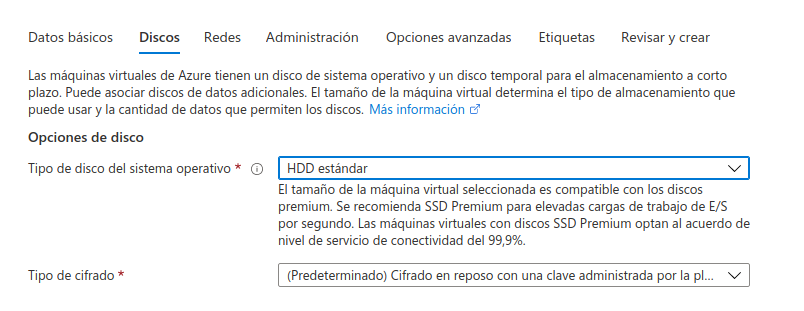
\includegraphics[scale=0.5]{imgs/creacion_3.png}\\
  \textit{Figura 3: Casillas de selección para la creación de la VM}\\
  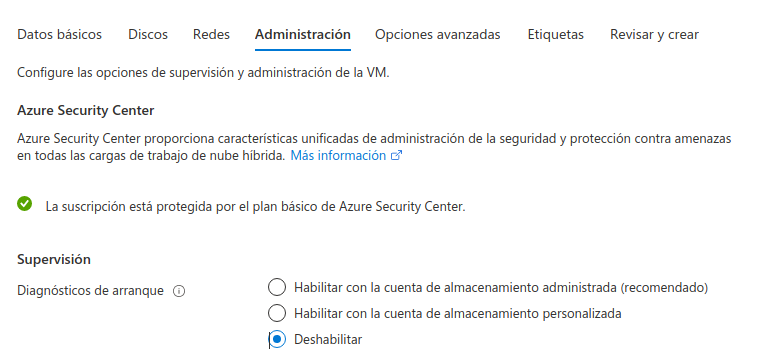
\includegraphics[scale=0.5]{imgs/creacion_4.png}\\
  \textit{Figura 4: Casillas de selección para la creación de la VM}\\
  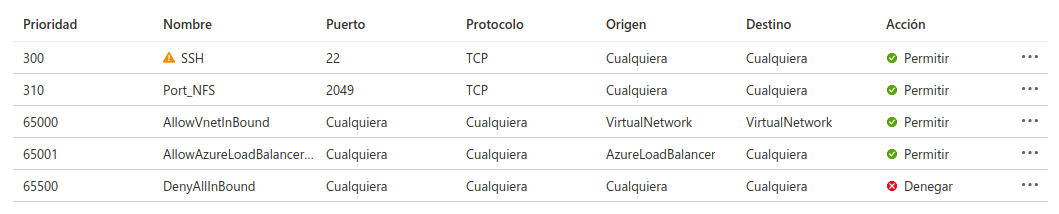
\includegraphics[scale=0.4]{imgs/conf_ports.png}\\
  \textit{Figura 5: Configuración de puertos para funcionamiento}
\end{center}
\subsection{En ejecución}
\begin{center}
  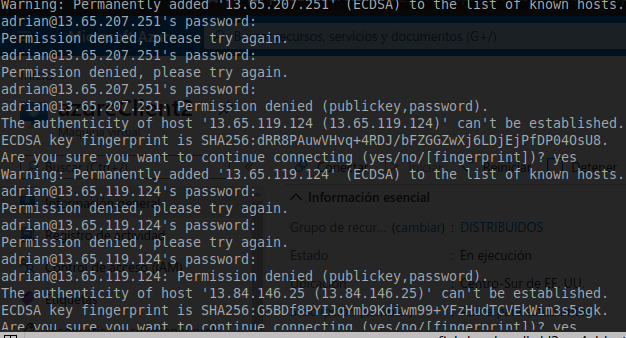
\includegraphics[scale=0.5]{imgs/first_con.png}\\
  \textit{Figura 6: Conexión inicial al servidor y cliente via ssh y ejecución remota de comandos}\\
  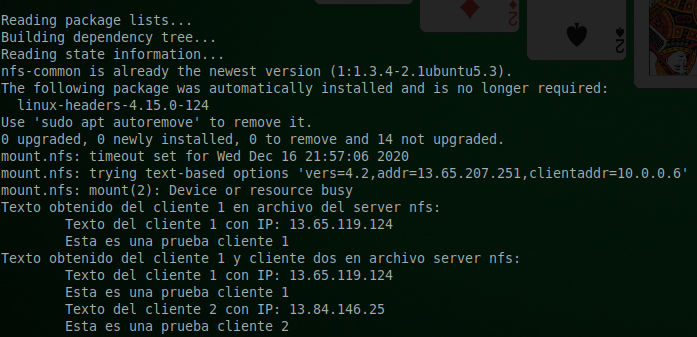
\includegraphics[scale=0.5]{imgs/ejecucion_script.png}\\
  \textit{Figura 7: Ejecución del primer script para la instalación de datos}\\
  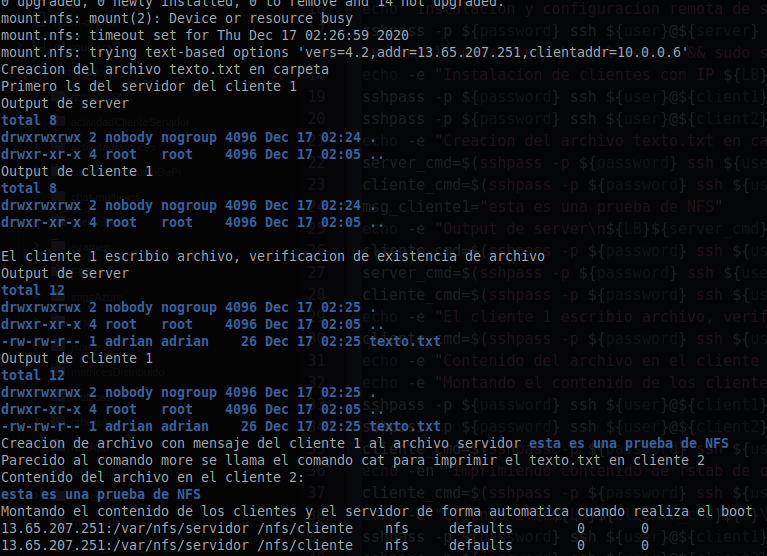
\includegraphics[scale=0.5]{imgs/script_archivo_contenido.png}\\
  \textit{Figura 8: Contenido de las siguientes instrucciones del script}\\
  \begin{landscape}
    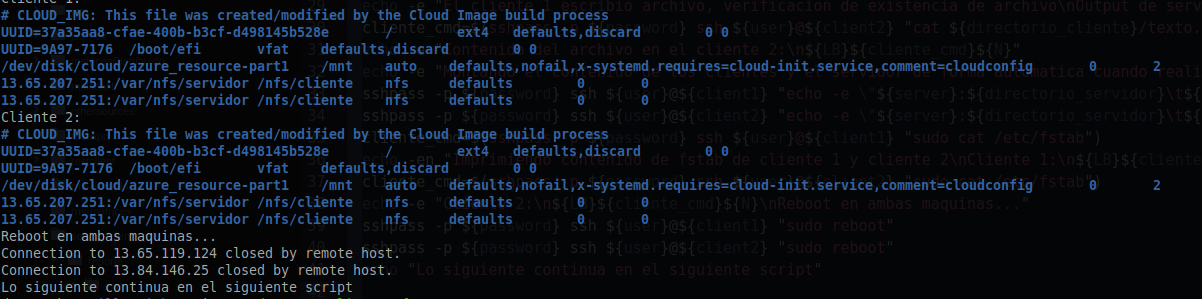
\includegraphics[scale=0.5]{imgs/boot_part.png}\\
    \textit{Figura 9: Contenido de las siguientes instrucciones del script en la parte donde añade los datos suficientes al fstab para el montado durante el boot}\\
    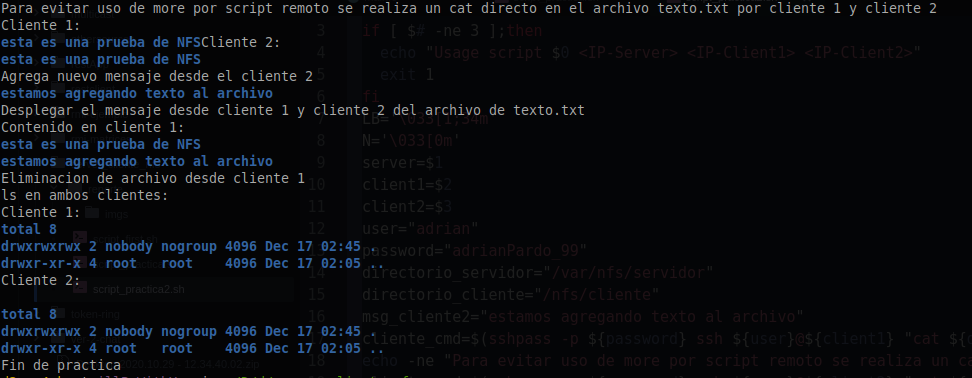
\includegraphics[scale=0.5]{imgs/script_final.png}\\
    \textit{Figura 10: Ejecución del ultimo script para las ultimas instrucciones despues del reboot sin necesidad de volver a montar los servicios de NFS}\\
    \fillandplacepagenumber
  \end{landscape}
\end{center}
\section{Conclusiones}
El hacer uso de NFS a nivel de sistemas distribuidos son muy importantes ya que nos permiten realizar una modifcación directa de datos a traves de la idea de cliente servidor, pero con la ayuda o el beneficio de que se pueda realizar vía distribuida para que muchos usuarios puedan acceder al recurso algunas aplicaciones que siguen esta idea para realizar trabajos de forma colaborativa es con aplicaciones como GitDuck o en plataformas de CodeShare que permiten trabajo colaborativo en el mismo espacio de trabajo.
\end{document}
